%tag:000Z
%label:"exr:biranCornea3ended"
%author:JeffHicks
%name:"surgery triangle from Lagrangian cobordism"
%type:"exercise"

 
 
Let $X$ be a compact symplectic manifold. Recall that a \emph{3-ended Lagrangian cobordism} $K: (L_0, L_1)\rightsquigarrow L_2$ is a closed Lagrangian submanifold $K\subset X\times \CC$ with the property that there exists a compact subset $U\subset \CC$ so that \[K|_{\pi_\CC^{-1}(\CC\setminus U)}=((L_0\times \RR_{>0})\cup( L_1\times (\sqrt{-1}+\RR_{>0}) )\cup( L_2\times (\RR_{<0})))|_{\pi_\CC^{-1}(\CC\setminus U)}.\]
Suppose that $X$ is an exact symplectic manifold, which in turn makes $X\times \CC$ an exact symplectic manifold. Let $K$ be an exact 3-ended Lagrangian cobordism. 
    %label:"fig:3EndedLagrangianCobordism"
%author:JeffHicks
%name:"3 ended Lagrangian cobordism"
%type:"figure"
%parent:"exr_biranCornea3ended"
%caption:"The projection to the $\CC$ coordinate of a 3-ended Lagrangian cobordism"


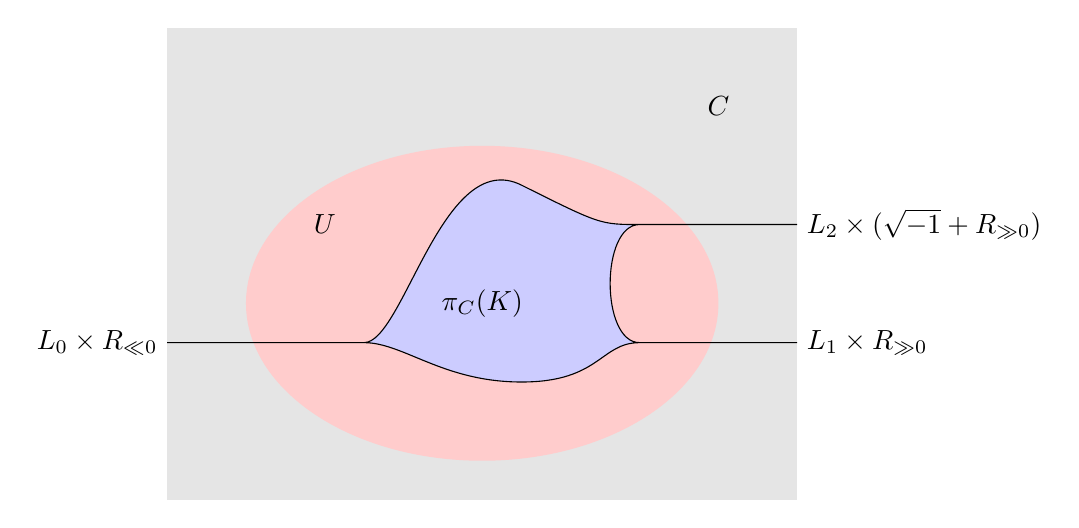
\begin{tikzpicture}

\fill[gray!20]  (-3.5,2.5) rectangle (4.5,-3.5);
\fill[fill=red!20]  (0.5,-1) ellipse (3 and 2);

\draw[fill=blue!20] (-3.5,-1.5) .. controls (-3,-1.5) and (-1.5,-1.5) .. (-1,-1.5) .. controls (-0.5,-1.5) and (0,-2) .. (1,-2) .. controls (2,-2) and (2,-1.5) .. (2.5,-1.5) .. controls (3,-1.5) and (4,-1.5) .. (4.5,-1.5) .. controls (4,-1.5) and (3,-1.5) .. (2.5,-1.5) .. controls (2,-1.5) and (2,0) .. (2.5,0) .. controls (3,0) and (4,0) .. (4.5,0) .. controls (4,0) and (3,0) .. (2.5,0) .. controls (2,0) and (2,0) ..(1,0.5) .. controls (0,1) and (-0.5,-1.5) .. (-1,-1.5);
\node[left] at (-3.5,-1.5) {$L_0\times \mathbb R_{\ll 0}$};
\node[right] at (4.5,-1.5) {$L_1\times \mathbb R_{\gg 0}$};
\node[right] at (4.5,0) {$L_2\times(\sqrt{-1}+ \mathbb R_{\gg 0})$};
\node at (0.5,-1) {$\pi_{\mathbb C}(K)$};
\node at (3.5,1.5) {$\mathbb C$};
\node at (-1.5,0) {$U$};
\end{tikzpicture}

\begin{enumerate}
    \item Show that $L_0, L_1$ and $L_2$ are exact Lagrangian submanifolds in $X$.
    \item Consider the curve $\gamma^-\subset \CC$. Show that for any exact Lagrangian submanifold $L\subset X$, $\CF(L\times \gamma^-, K)=\CF(L, L_0)$ as a vector space. 
    \item Give $X\times \CC$ an almost complex structure of the form $J_X\times J_\CC$. Suppose that we have a finite energy pseudoholomorphic strip $u: \RR\times [0, 1]\to X\times \CC$ with $u(t, 0)\in L\times \gamma^-$ and $u(t, 1)\in K$, and ends limiting to intersections of $L\times \gamma^-\cap K$. Show that $\pi_\CC(u)\in \text{Im}(\gamma^-)\cap \RR_{<0}$ (the location of the red cross in the figure). From this, conclude that if $J_X$ is chosen so that all pseudoholomorphic strips with boundary on $L, L_2$ are regular, that $\CF(L\times \gamma^-, K) = \CF(L_2, K)$ \emph{as chain complexes}.
        %label:"fig:3EndedLagrangianCobordismGammaMinus"
%author:JeffHicks
%name:"3 ended Lagrangian cobordism with curve $\gamma^-$"
%type:"figure"
%parent:"exr_biranCornea3ended"
%caption:"Profile of the curve $\gamma^-$"


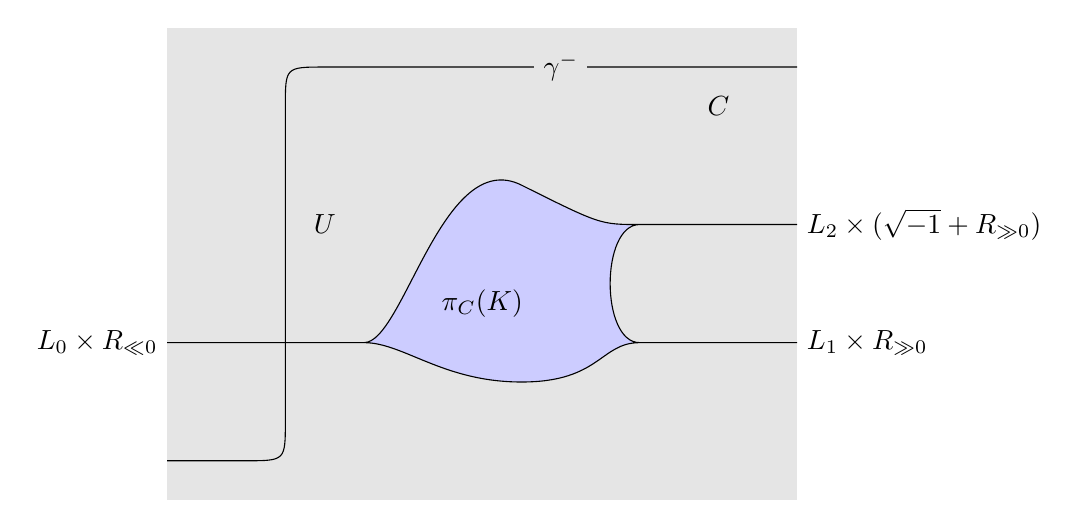
\begin{tikzpicture}

\fill[gray!20]  (-3.5,2.5) rectangle (4.5,-3.5);

\draw[fill=blue!20] (-3.5,-1.5) .. controls (-3,-1.5) and (-1.5,-1.5) .. (-1,-1.5) .. controls (-0.5,-1.5) and (0,-2) .. (1,-2) .. controls (2,-2) and (2,-1.5) .. (2.5,-1.5) .. controls (3,-1.5) and (4,-1.5) .. (4.5,-1.5) .. controls (4,-1.5) and (3,-1.5) .. (2.5,-1.5) .. controls (2,-1.5) and (2,0) .. (2.5,0) .. controls (3,0) and (4,0) .. (4.5,0) .. controls (4,0) and (3,0) .. (2.5,0) .. controls (2,0) and (2,0) ..(1,0.5) .. controls (0,1) and (-0.5,-1.5) .. (-1,-1.5);
\node[left] at (-3.5,-1.5) {$L_0\times \mathbb R_{\ll 0}$};
\node[right] at (4.5,-1.5) {$L_1\times \mathbb R_{\gg 0}$};
\node[right] at (4.5,0) {$L_2\times(\sqrt{-1}+ \mathbb R_{\gg 0})$};
\node at (0.5,-1) {$\pi_{\mathbb C}(K)$};
\node at (3.5,1.5) {$\mathbb C$};
\node at (-1.5,0) {$U$};
\draw (-3.5,-3) .. controls (-3,-3) and (-3,-3) .. (-2.5,-3) .. controls (-2,-3) and (-2,-3) .. (-2,-2.5) .. controls (-2,-2) and (-2,1) .. (-2,1.5) .. controls (-2,2) and (-2,2) .. (-1.5,2) .. controls (-1,2) and (4,2) .. (4.5,2);
\node[fill=gray!20] at (1.5,2) {$\gamma^-$};
\end{tikzpicture}
    \item Consider now the curve $\gamma^+\subset \CC$. Using a similar argument, one can prove that there are no pseudoholomorphic strips $u:\RR\times [0, 1]\to X\times \CC$ with $\lim_{t\to\infty} u(s, t)=z_2$ and $\lim_{t\to-\infty} u(s, t)=z_0$. What can you conclude about the relationship between $\CF(L\times \gamma^+, K)$, $\CF(L, L_0)$ and $\CF(L, L_1)$?
        %tag:000X
%label:"fig:3EndedLagrangianCobordismGammaPlus"
%author:JeffHicks
%name:"3 ended Lagrangian cobordism with curve $\gamma^+$"
%type:"figure"
%parent:exr_biranCornea3ended
%caption:"Profile of the curve $\gamma^+$"


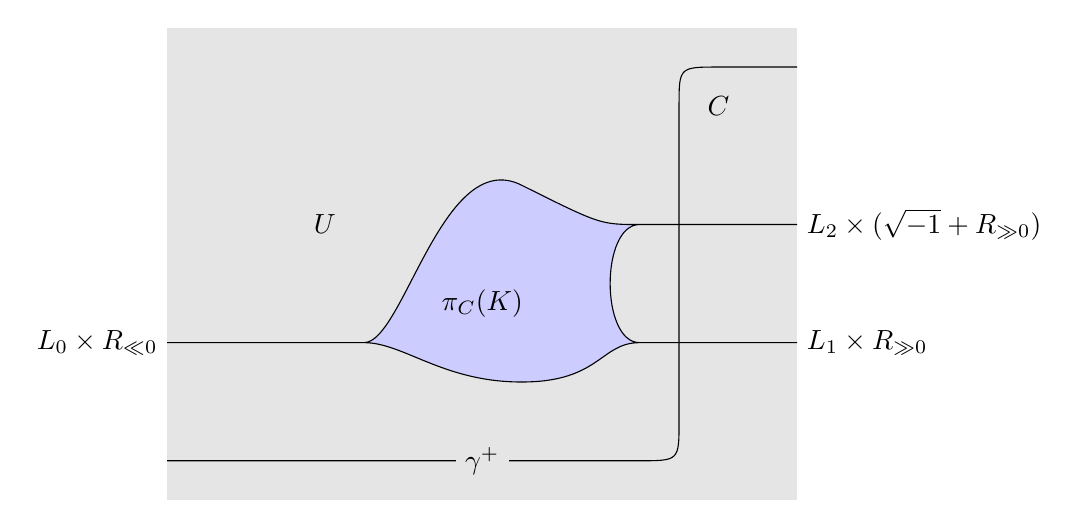
\begin{tikzpicture}

\fill[gray!20]  (-3.5,2.5) rectangle (4.5,-3.5);

\draw[fill=blue!20] (-3.5,-1.5) .. controls (-3,-1.5) and (-1.5,-1.5) .. (-1,-1.5) .. controls (-0.5,-1.5) and (0,-2) .. (1,-2) .. controls (2,-2) and (2,-1.5) .. (2.5,-1.5) .. controls (3,-1.5) and (4,-1.5) .. (4.5,-1.5) .. controls (4,-1.5) and (3,-1.5) .. (2.5,-1.5) .. controls (2,-1.5) and (2,0) .. (2.5,0) .. controls (3,0) and (4,0) .. (4.5,0) .. controls (4,0) and (3,0) .. (2.5,0) .. controls (2,0) and (2,0) ..(1,0.5) .. controls (0,1) and (-0.5,-1.5) .. (-1,-1.5);
\node[left] at (-3.5,-1.5) {$L_0\times \mathbb R_{\ll 0}$};
\node[right] at (4.5,-1.5) {$L_1\times \mathbb R_{\gg 0}$};
\node[right] at (4.5,0) {$L_2\times(\sqrt{-1}+ \mathbb R_{\gg 0})$};
\node at (0.5,-1) {$\pi_{\mathbb C}(K)$};
\node at (3.5,1.5) {$\mathbb C$};
\node at (-1.5,0) {$U$};
\draw (-3.5,-3) .. controls (2,-3) and (2,-3) .. (2.5,-3) .. controls (3,-3) and (3,-3) .. (3,-2.5) .. controls (3,-2) and (3,1) .. (3,1.5) .. controls (3,2) and (3,2) .. (3.5,2) .. controls (4,2) and (4,2) .. (4.5,2);
\node[fill=gray!20] at (0.5,-3) {$\gamma^+$};
\end{tikzpicture}
    \item Observe that $L\times \gamma^-$ and $L\times \gamma^+$ are Hamiltonian isotopic. Exhibit a long exact sequence whose terms are $\HF(L, L_0), \HF(L, L_1)$ and $\HF(L, L_2)$.
\end{enumerate}

 